%!TEX program = xelatex

\documentclass[compress]{beamer}
%--------------------------------------------------------------------------
% Common packages
%--------------------------------------------------------------------------

\definecolor{links}{HTML}{663000}
\hypersetup{colorlinks,linkcolor=,urlcolor=links}

\usepackage[english]{babel}
\usepackage{pgfpages} % required for notes on second screen
\usepackage{graphicx}

\usepackage{multicol}


\usepackage{tabularx,ragged2e}
\usepackage{booktabs}

\setlength{\emergencystretch}{3em}  % prevent overfull lines
\providecommand{\tightlist}{%
  \setlength{\itemsep}{0pt}\setlength{\parskip}{0pt}}


\usetheme{hri}

\usepackage{remreset}% tiny package containing just the \@removefromreset command
\makeatletter
\@removefromreset{subsection}{section}
\makeatother
\setcounter{subsection}{1}

\makeatletter
\let\beamer@writeslidentry@miniframeson=\beamer@writeslidentry
\def\beamer@writeslidentry@miniframesoff{%
  \expandafter\beamer@ifempty\expandafter{\beamer@framestartpage}{}% does not happen normally
  {%else
    % removed \addtocontents commands
    \clearpage\beamer@notesactions%
  }
}
\newcommand*{\miniframeson}{\let\beamer@writeslidentry=\beamer@writeslidentry@miniframeson}
\newcommand*{\miniframesoff}{\let\beamer@writeslidentry=\beamer@writeslidentry@miniframesoff}
\makeatother


\newcommand{\source}[2]{{\tiny\it Source: \href{#1}{#2}}}

\usepackage{tikz}
\usetikzlibrary{mindmap,backgrounds,positioning}

\graphicspath{{figs/}}

\title{ROCO222 \newline Intro to Sensors and Actuators}
\subtitle{Introduction, Arduinos and Encoders}
\date{}
\author{Séverin Lemaignan}
\institute{Centre for Neural Systems and Robotics\\{\bf Plymouth University}}

\begin{document}

\licenseframe{github.com/severin-lemaignan/module-introduction-sensors-actuators}

\maketitle


\begin{frame}{Who am I?}

\begin{center}
    \textbf{Séverin Lemaignan}, B316 Portland Square
\end{center}

\begin{multicols}{2}

    \textbf{Cognitive robotics}

  Building robots and their artificial intelligence inspired on natural
  systems, such as developing children

    \textbf{Human-Robot Interaction}

  Building robots that can work alongside people, using social cues that
  people use to communicate

    \begin{center}
        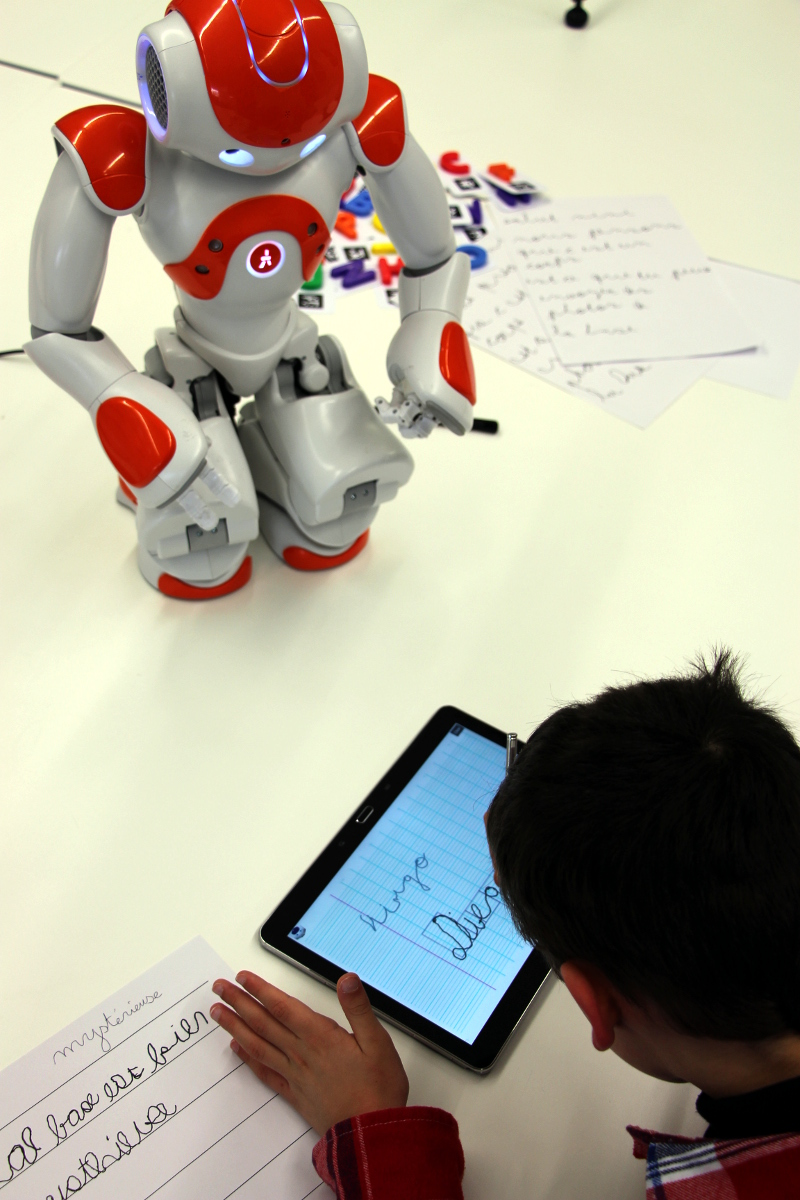
\includegraphics[width=0.7\linewidth]{cowriter}
    \end{center}

\end{multicols}
\end{frame}

\begin{frame}{Availability}

    \begin{itemize}
        \item I have lots of time (2 hours) to deal with your queries in the laboratory sessions
        \item  Otherwise, the best thing to do is to email me first and see if I can sort out your query. If not then I will arrange a time to meet up with you.
        \item Don't forget – if you have any problems, or even if you are not sure about something - just email me

    \end{itemize}

    \begin{center}
        \texttt{severin.lemaignan@plymouth.ac.uk}
    \end{center}
\end{frame}

\begin{frame}{Registration}
        \centering
        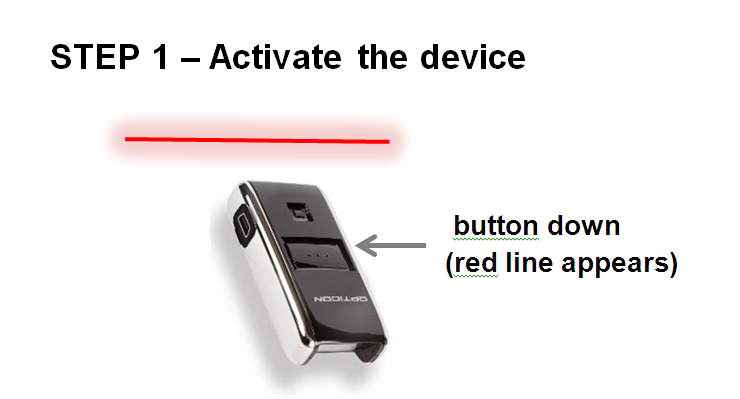
\includegraphics[width=0.4\linewidth]{registration1}
        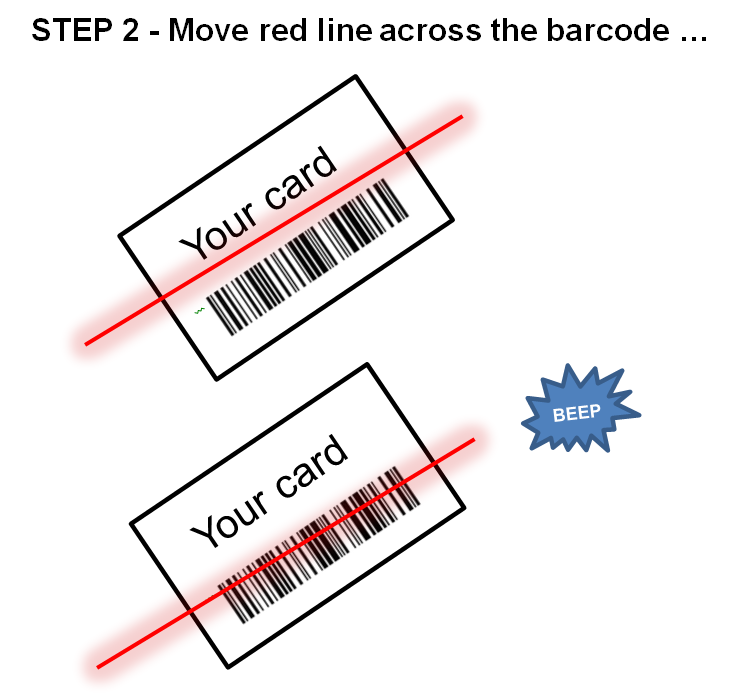
\includegraphics[width=0.4\linewidth]{registration2}
\end{frame}

\begin{frame}{Special needs}

    \begin{itemize}

    \item Anyone with dyslexia or any other special needs that requires any form
        of support during examinations and tests should email me immediately.

    \item Please do not ASSUME that I know of your condition. It takes the
        University some weeks to process data and forward it to the correct
            members of staff.

    \item Even if you are currently undergoing assessment, it is advisable to
        contact me and I will organize suitable support for you during your
            tests and exams.

    \item Contact me if any issues relating to harassment, inclusivity or if
        language/cultural difficulties arise.

    \end{itemize}
\end{frame}

\begin{frame}{Labs}
    \begin{itemize}
        \item ROCO222 is also taught and supervised in a computer laboratory for
            TWO HOURS EACH WEEK.
        \item There are 2 labs so please go to your timetabled group and pair up
            with someone
    \end{itemize}

    \centering
          \begin{tabular}{@{}llll@{}}
                \toprule
                Day?                & Time? & Where?   & Who? \\ \midrule
                Monday -- Lab 1/\textbf{02} & 09:00--11:00     & SMB 307  & Jake \& myself            \\
                Thursday -- Lab 1/\textbf{01} & 11:00--13:00     & SMB 307  & Jake \& myself          \\ \bottomrule
            \end{tabular}


\end{frame}

\section[]{Assessment}

\begin{frame}{Assessment}
    \begin{exampleblock}{Formative vs Summative}
        \textbf{Formative}: during the term; \textbf{Summative}: at the end of
        the term.
    \end{exampleblock}

    \begin{itemize}
        \item There will be practical assessments in the form of laboratory
            practical work (60\%)
        \item \textbf{First practical needs to be submitted by 16:00, 13th October 2017}
        \item Feedback within 20 working days
        \item Complete lab journal submitted \textbf{Thursday 16:00, 11th January 2018}
        \item There will be a final written exam (40\%) -- \textbf{note that the
            exam questions may touch upon material discussed during the labs}
    \end{itemize}

\end{frame}


\section[]{Robotics: what are your expectations?}

\begin{frame}[plain]
    \begin{center}
        \Large
    \href{https://www.mentimeter.com/s/d42456cc370aa465642c7e815a68646b/4fdc61757b92}{Go to www.menti.com and use the code 60 34 45}
    \end{center}
\end{frame}


\section[Overview]{Module Overview}

\videoframe[0.56]{figs/NISSAN-ProPILOT-chair.mp4}


\begin{frame}{Module aims}
    \begin{itemize}
        \item<+-> Develop an in-depth understanding of \textbf{what electrical motors are},
            \textbf{how they work} (hands-on!), how they are characterised
        \item<+-> Learn how to \textbf{control them}, and \textbf{program an embedded controller}
            for your own motor
        \item<+-> Get a first \textbf{hand-on experience with a complete robotic system}:
            from the hardware, to the low-level closed-loop control, to
            system-level programming and visualisation
        \item<+-> \textbf{We have a bit of room to touch additional topics}
    \end{itemize}
\end{frame}

\begin{frame}{Learning outcomes}
    \begin{enumerate}
        \item<+-> Demonstrate knowledge and critical understanding of the operating
            \textbf{characteristics of electrical motors} (brushed, brushless,
            servo, stepper motors...)
        \item<+-> Explore (some) \textbf{robot sensors}, integrate them into software
        \item<+-> Comprehend and characterise the effects of \textbf{closing the speed and current
            loops} in drive systems; demonstrate it practically by \textbf{creating a
            closed loop motor system}
        \item<+-> Understand the fundamentals of the \textbf{ROS middleware},
            and use it to control motors and run simple robot visualisations
        \item<+-> Acquire the \textbf{basics of software engineering}; feel
            confident when using the \textbf{Linux command-line}; know how to
            use and reflect on \textbf{document/code versioning and sharing}
            (with git)

    \end{enumerate}
\end{frame}

\begin{frame}{In your curriculum}
    \begin{itemize}
        \item Last year: quite a lot of electronics, \textbf{ROCO103PP}?
        \item Next term: \textbf{ROCO224} (Martin Stoelen) -- kinematics, mechanical engineering,
            robot control
        \item Next year: \textbf{ROCO318} -- sensors, algorithms, AI (path
            planning, localisation)
    \end{itemize}
\end{frame}


\begin{frame}{This year: ROCO222 and ROCO224}

    \only<1>{
    \Large
    \textbf{From...}

    \begin{center}
        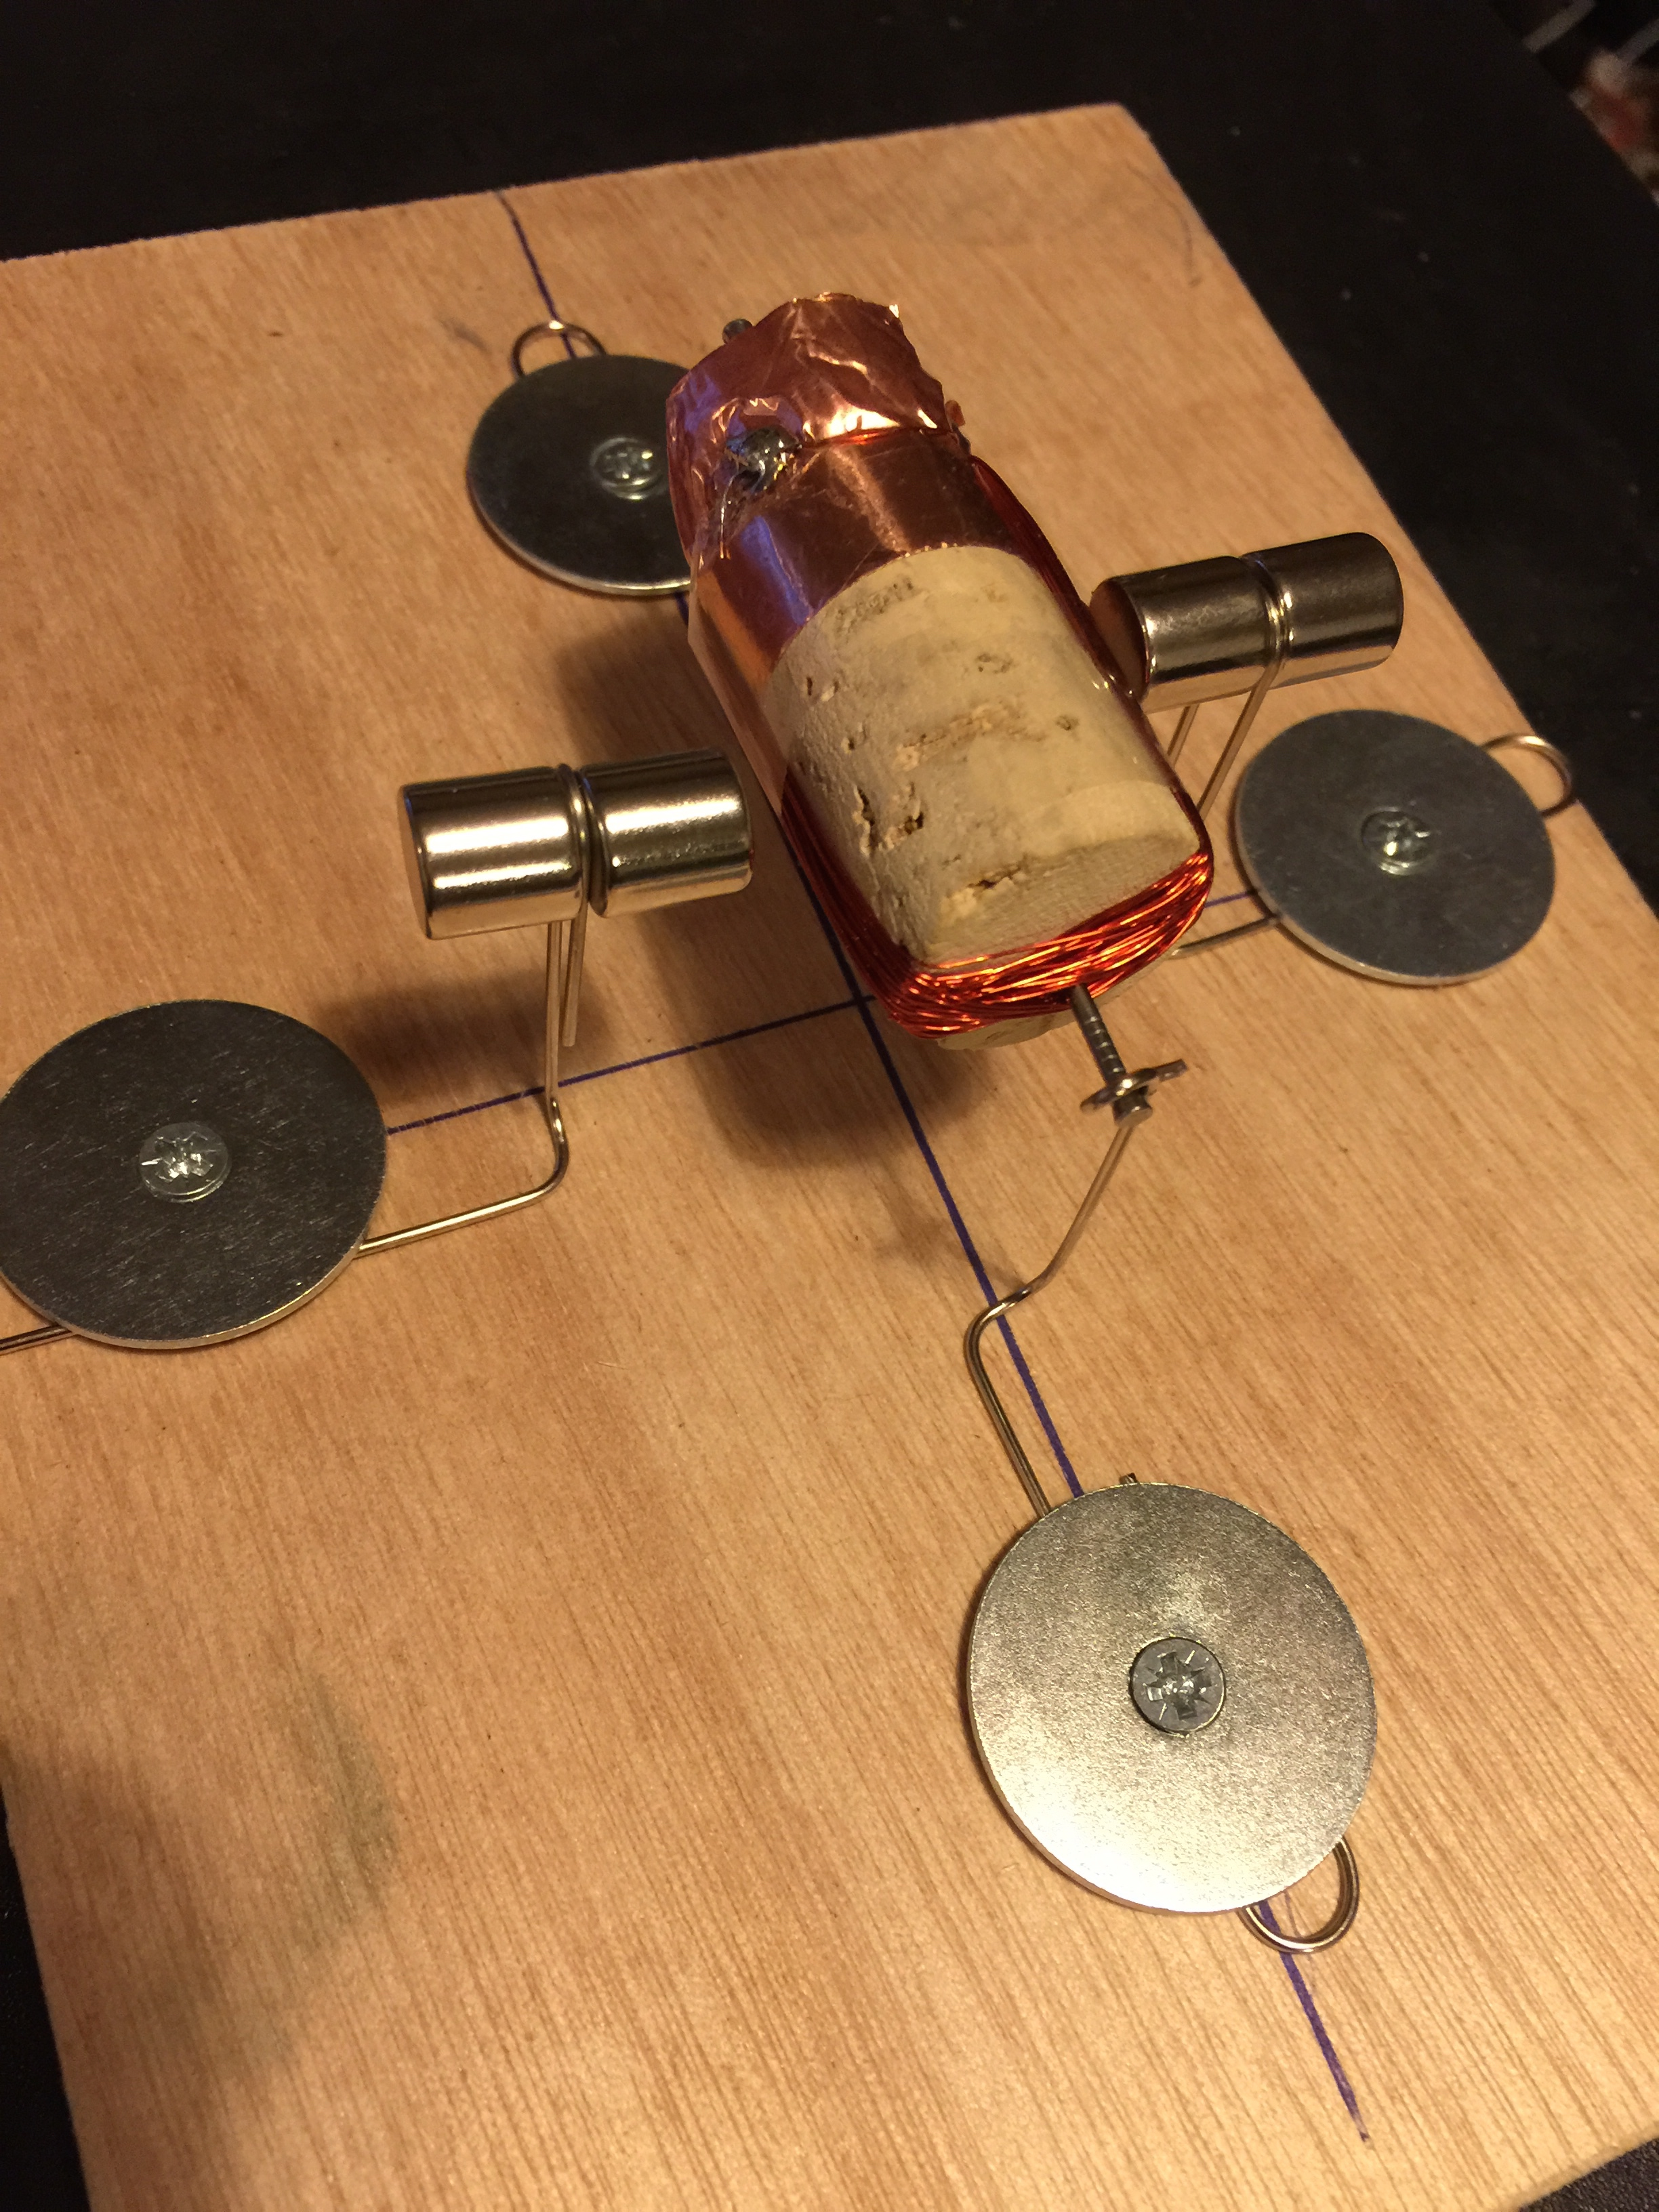
\includegraphics[width=0.5\paperheight]{better-dc-motor}
    \end{center}

    }
    \only<2> {
        \Large
    \textbf{...to}

    \begin{center}
        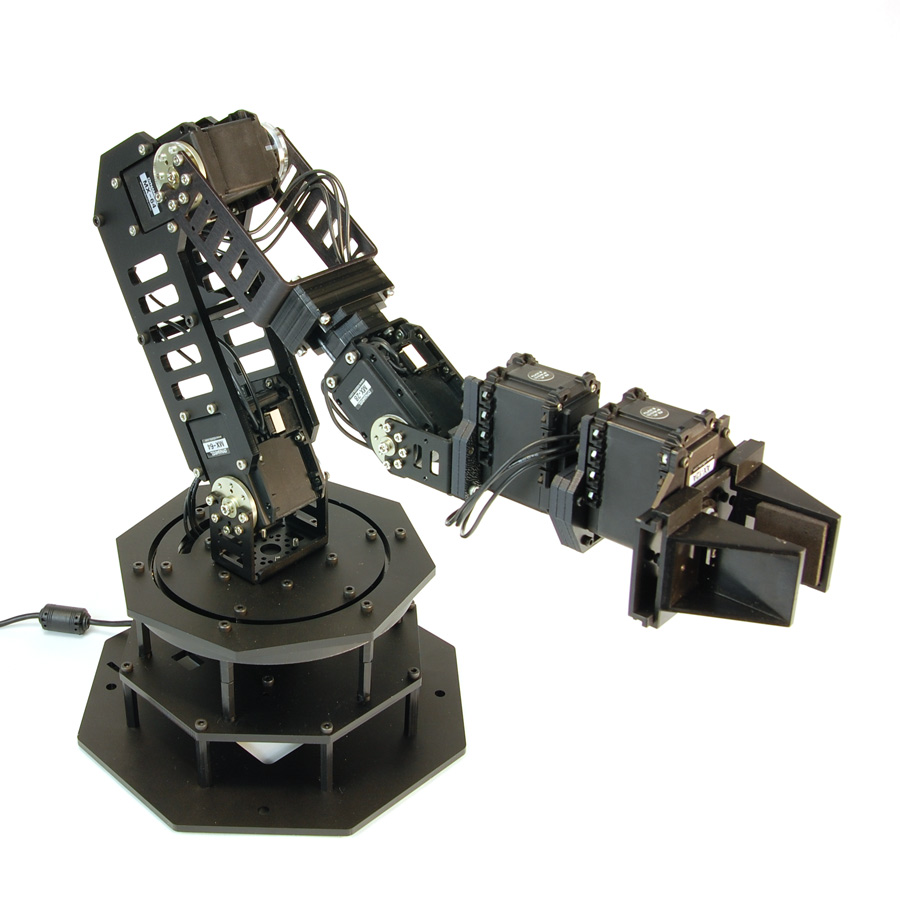
\includegraphics[width=0.6\paperheight]{servo-arm}
    \end{center}

    }

\end{frame}

\begin{frame}{This module: syllabus}

\begin{itemize}
    \item<+-> \textbf{Week 1} -- Arduino + Encoders
    \item<+-> \textbf{Week 2} -- The physics behind motors: electromagnetism, induction, magnetic
        force
    \item<+-> \textbf{Week 4} -- DC motors, brushed \& brushless
    \item<+-> \textbf{Week 5} -- Closed-loop motor control, PWM, PID, H-bridge
    \item<+-> \textbf{Week 6} -- Induction motors
    \item<+-> \textbf{Week 7} -- Servo-motors \& stepper motors
    \item<+-> \textbf{Week 9} -- Software engineering for robotics
    \item<+-> \textbf{Week 10} -- ROS middleware, joint state, kinematics 101, visualisation
    \item<+-> \textbf{Week 11} -- Sensors
\end{itemize}

\end{frame}

\section[Labs]{Laboratory Coursework}

\begin{frame}{This week: Lab journal \& Command-line 101}
    \begin{itemize}
        \item Document versioning: what is GIT?
        \item Creating \& managing a lab journal with GIT and markdown
        \item Linux command-line
        \item Remotely connecting to a robot
    \end{itemize}

    \begin{exampleblock}{Tomorrow's practical}
        If you want to, you can come from 11:00 to 13:00 to finish Monday's
        practical (including connecting to the robot)
    \end{exampleblock}



\end{frame}

\begin{frame}{Build a DC motor}
    \begin{columns}
        \begin{column}{0.45\linewidth}
            Build a DC brushed motor from first principles
            \begin{itemize}

                \item Wind armature

                \item Position field magnets

                \item Build commutator

                \item Test operation

                \item Measure characteristics

            \end{itemize}

        \end{column}
        \begin{column}{0.45\linewidth}

            \begin{center}
                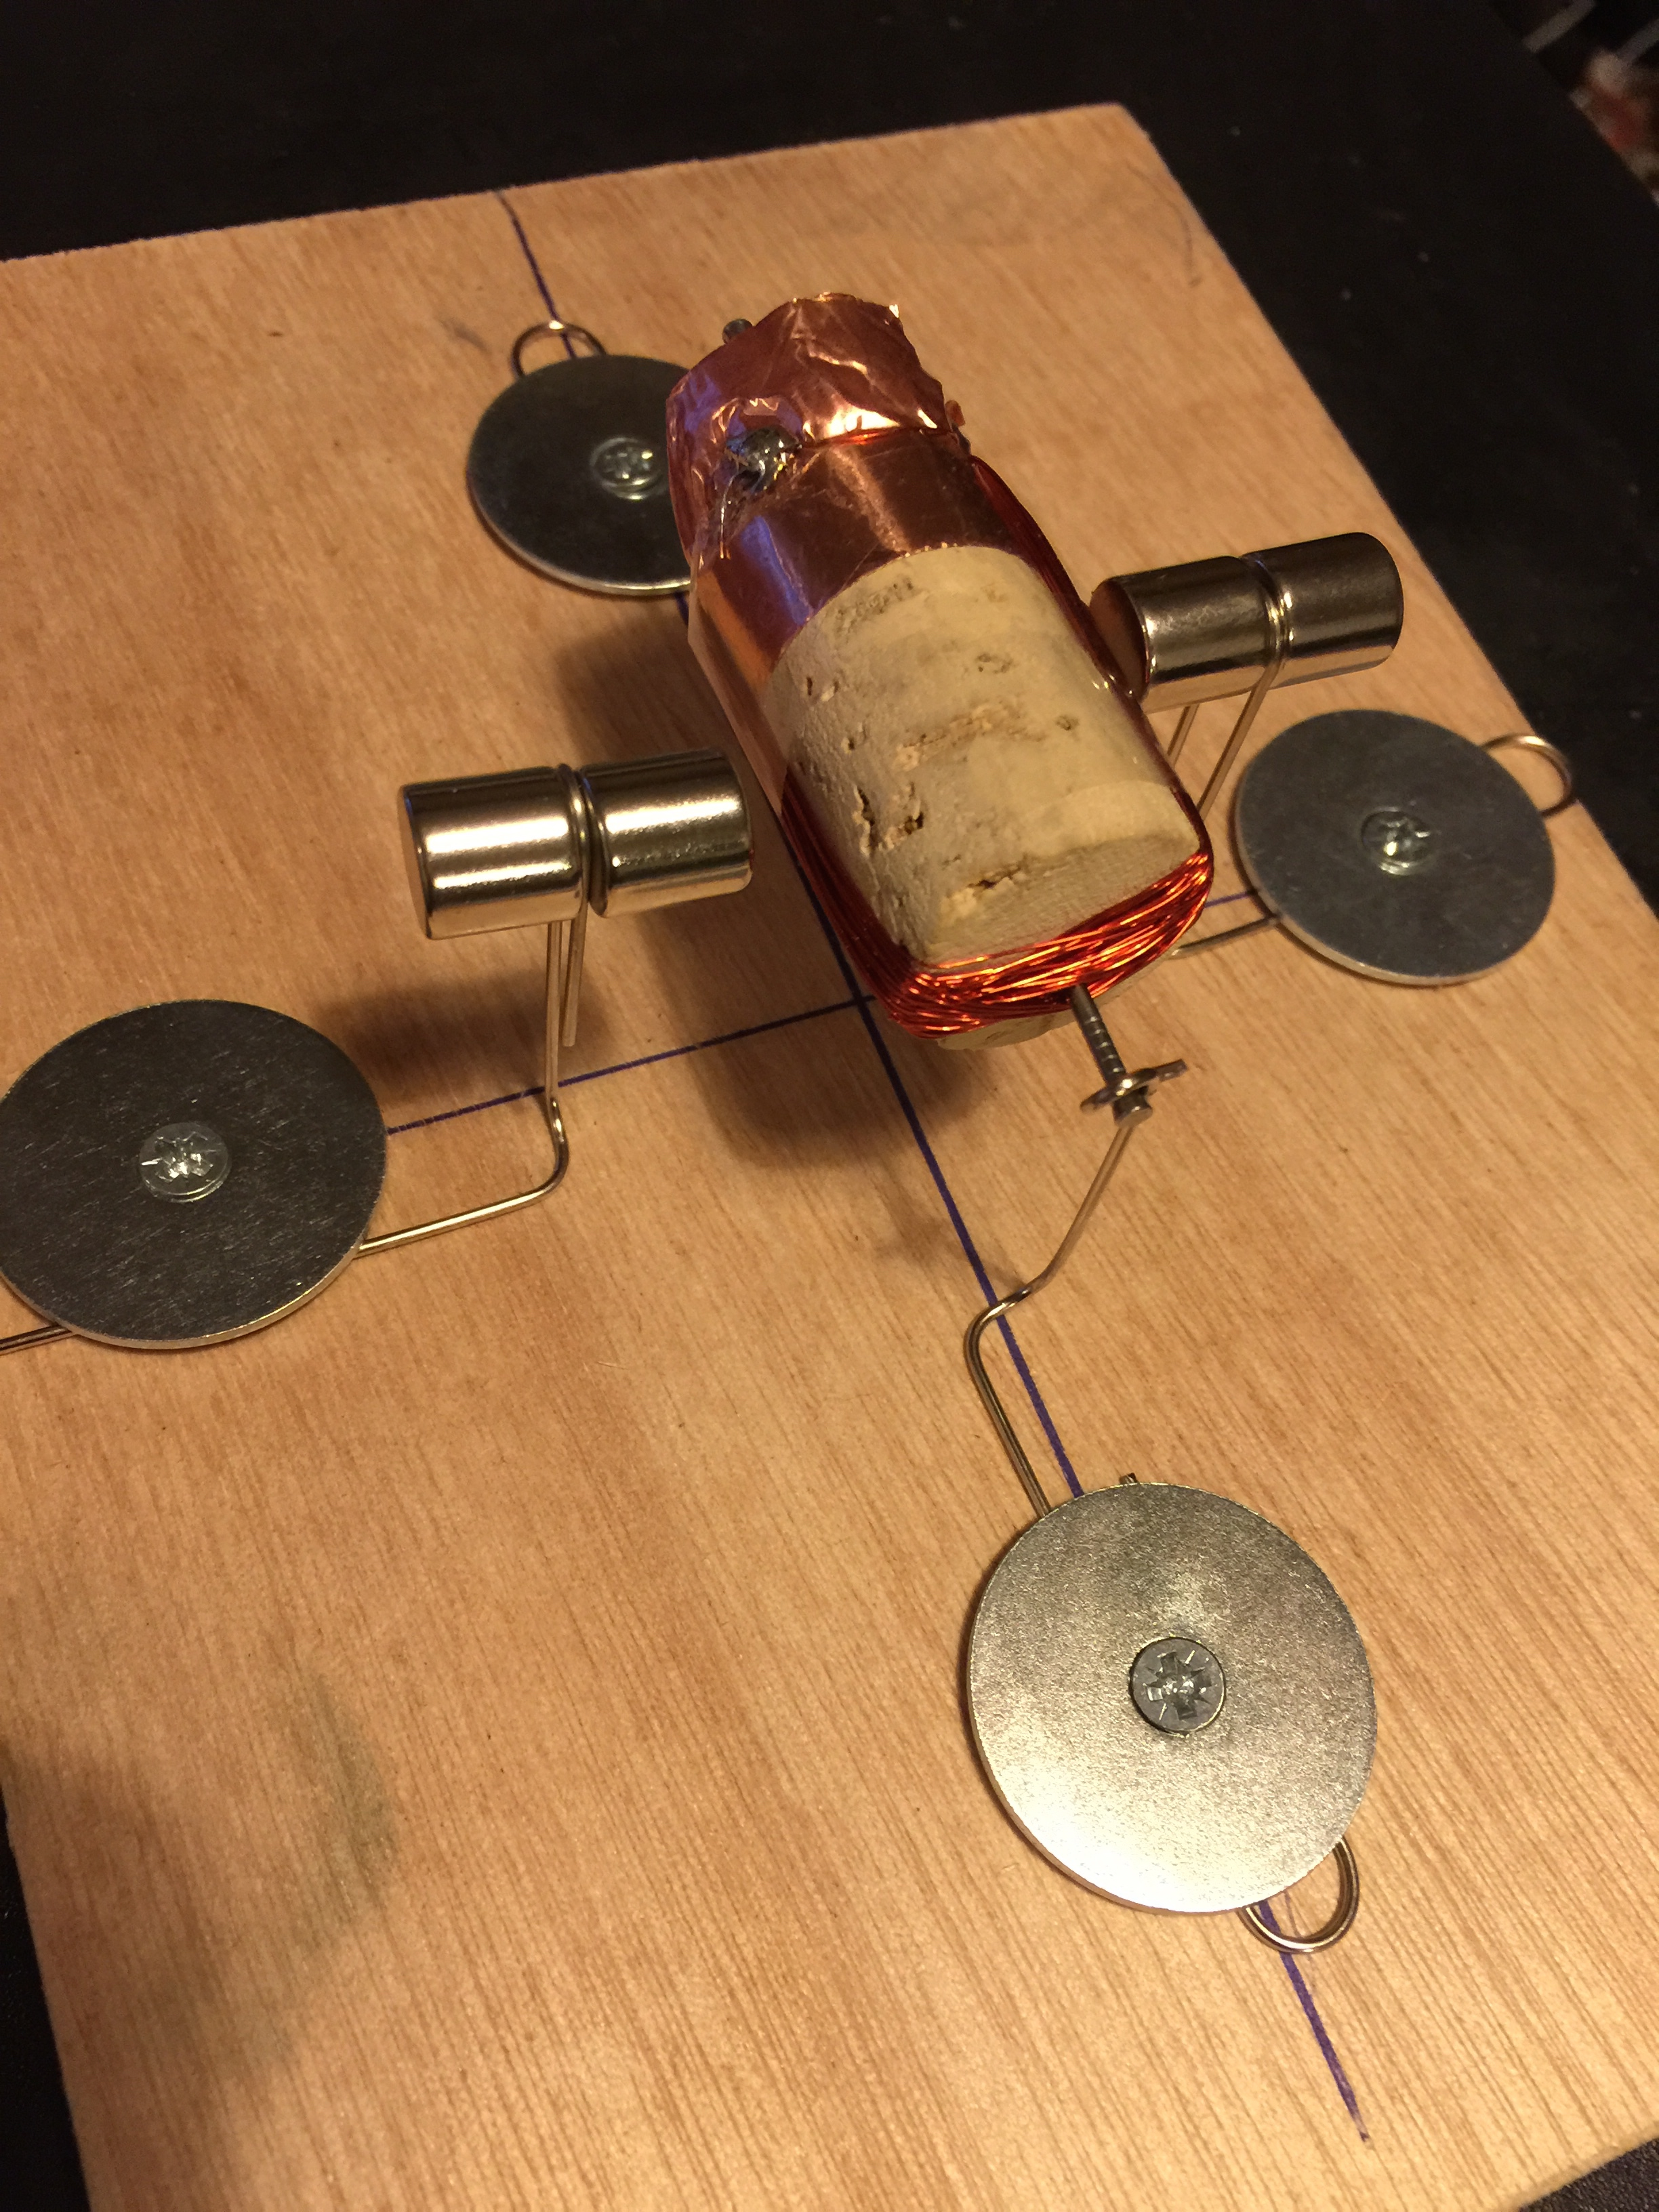
\includegraphics[width=0.6\columnwidth]{better-dc-motor}\\
                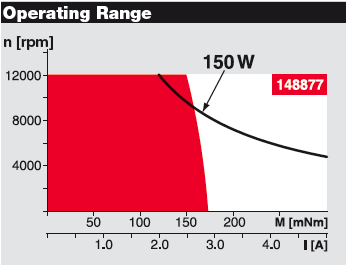
\includegraphics[width=0.8\columnwidth]{motor-characterisation}
            \end{center}

        \end{column}
    \end{columns}
\end{frame}

\begin{frame}{Introduction to Arduino and simple motor control}
    \begin{columns}
        \begin{column}{0.45\linewidth}

            \begin{itemize}
                \item Controlling your DC motor using an Arduino
                \item Build a speed-controlled electric fan \eg use
                    temperature sensor

                \item Control an RC servo using an Arduino
            \end{itemize}
        \end{column}
        \begin{column}{0.45\linewidth}

            \begin{center}
                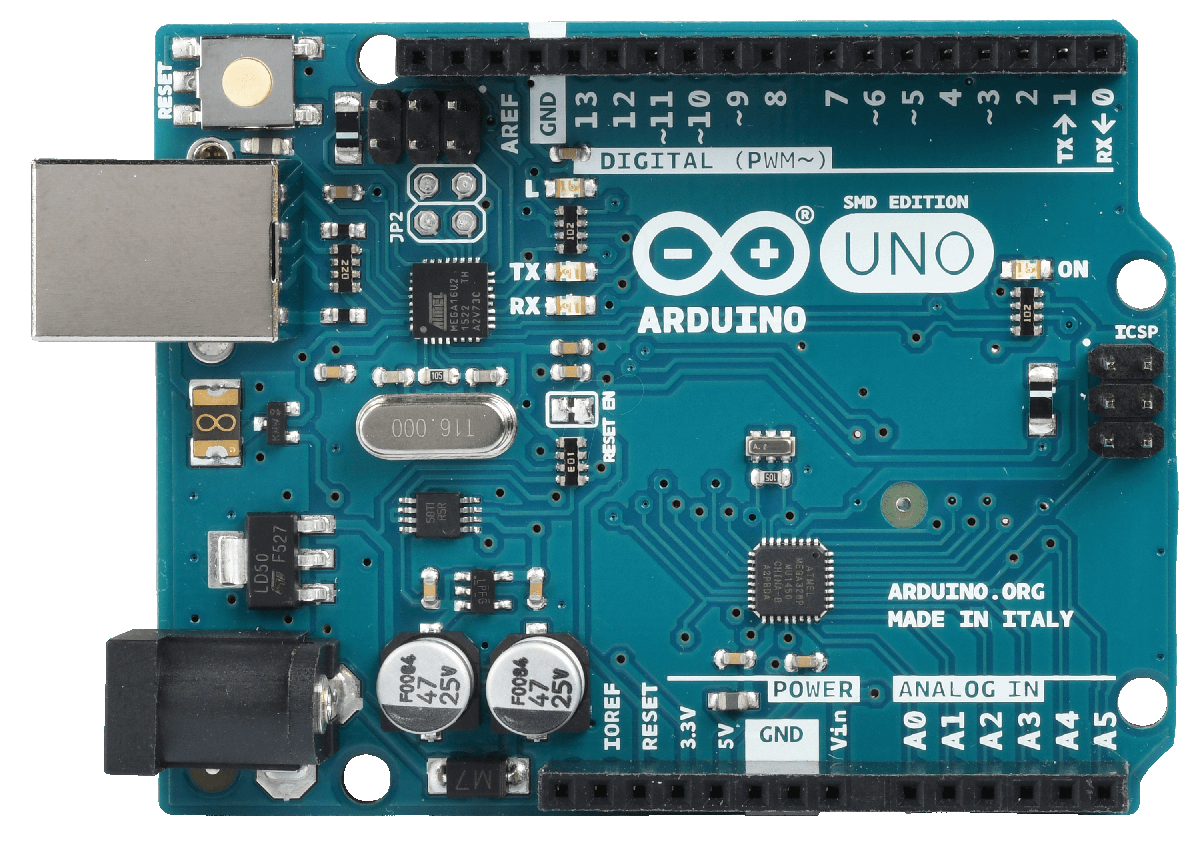
\includegraphics[width=0.8\columnwidth]{arduino-uno}\\
                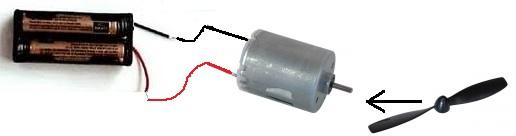
\includegraphics[width=0.8\columnwidth]{dc-motor-fan}\\
                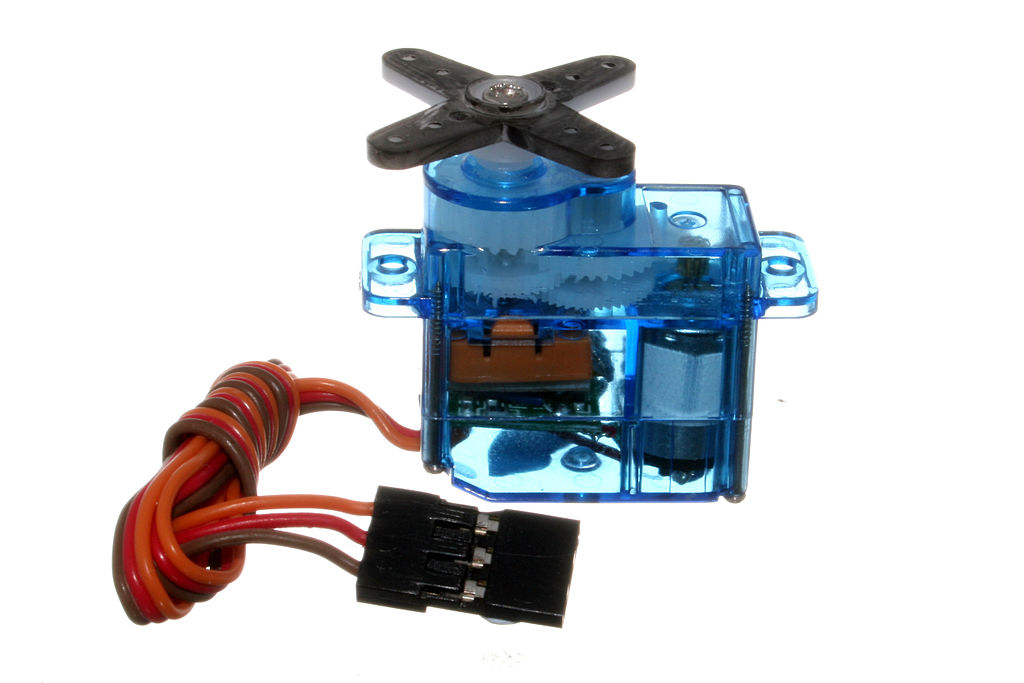
\includegraphics[width=0.8\columnwidth]{servo}\\
            \end{center}

        \end{column}
    \end{columns}
\end{frame}


\begin{frame}{Build an incremental encoder}
    \begin{columns}
        \begin{column}{0.45\linewidth}

            \begin{itemize}
                    \item Build a simple encoder from first principles
                    \item Use a LED and phototransistor
                    \item Measure rotational speed of a small DC motor
                    \item Integrate it with the Arduino
            \end{itemize}
        \end{column}
        \begin{column}{0.45\linewidth}

            \begin{center}
                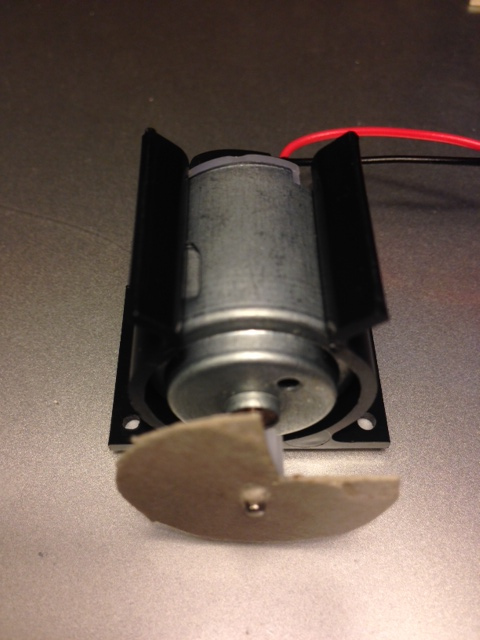
\includegraphics[width=0.9\columnwidth]{encoder}\\
            \end{center}

        \end{column}
    \end{columns}
\end{frame}


\begin{frame}{Write a PID controller for your DC motor}
    \begin{center}
        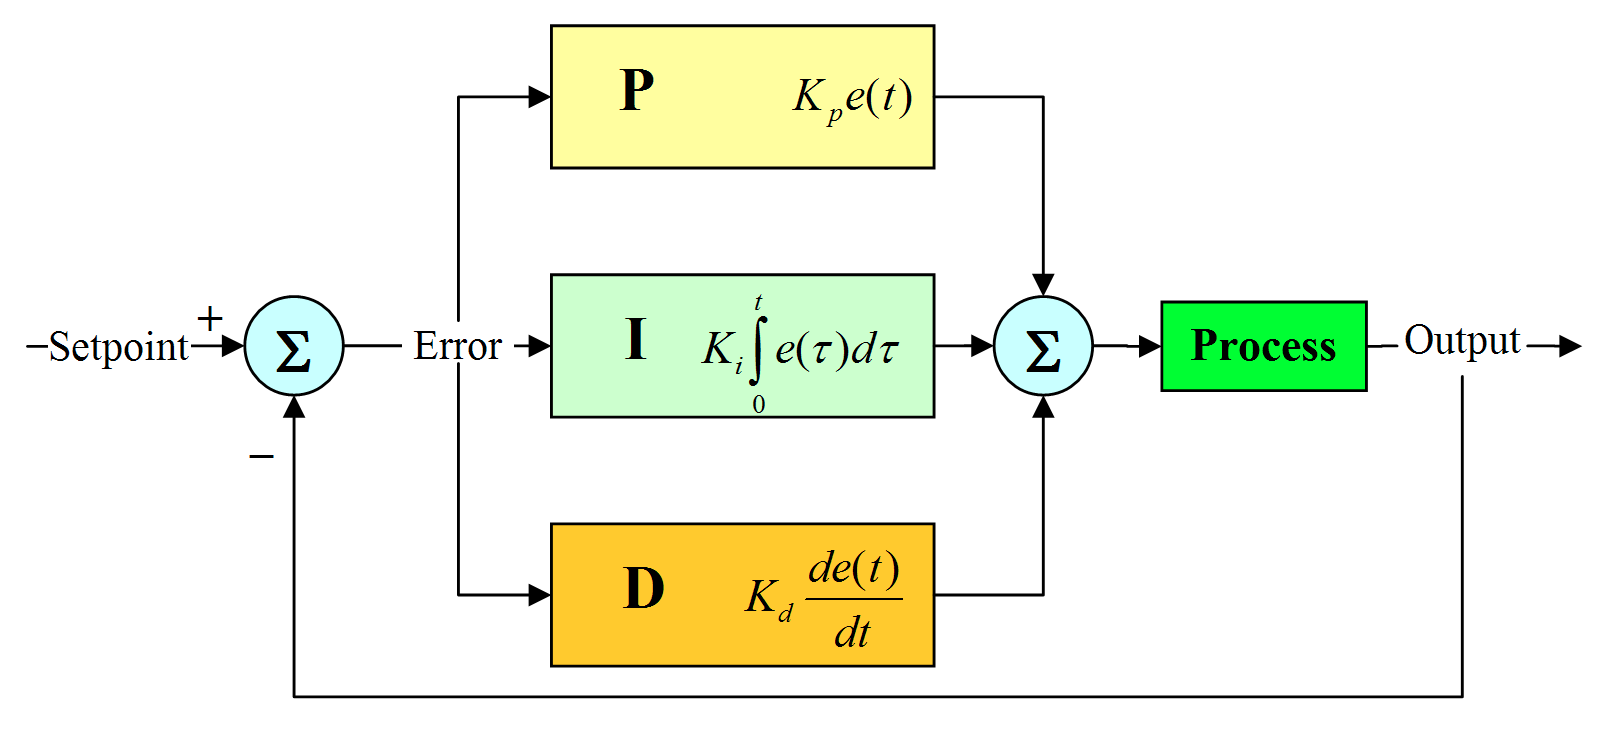
\includegraphics[width=0.8\linewidth]{pid}
    \end{center}
\end{frame}

\begin{frame}{Control a stepper motor with an Arduino}
    \begin{center}
        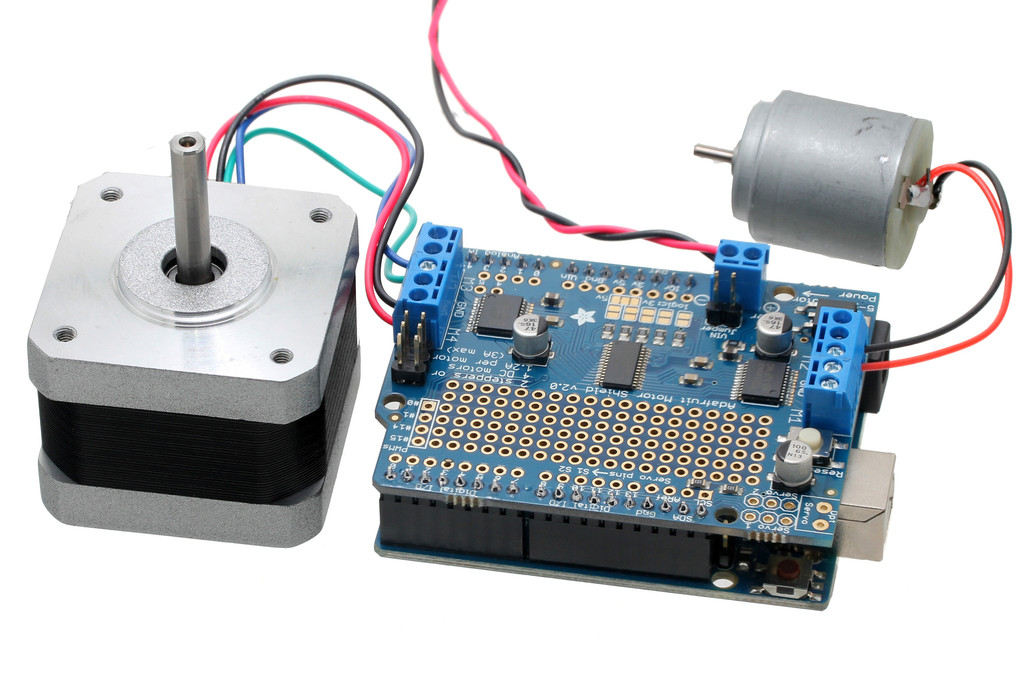
\includegraphics[width=0.8\linewidth]{stepper}
    \end{center}

    \begin{itemize}
        \item Control a stepper motor from the Arduino
        \item Implement stepper modes from first principles
    \end{itemize}
\end{frame}

\begin{frame}{Mini project: a 3DoF robot arm controlled from ROS}
    \begin{center}
        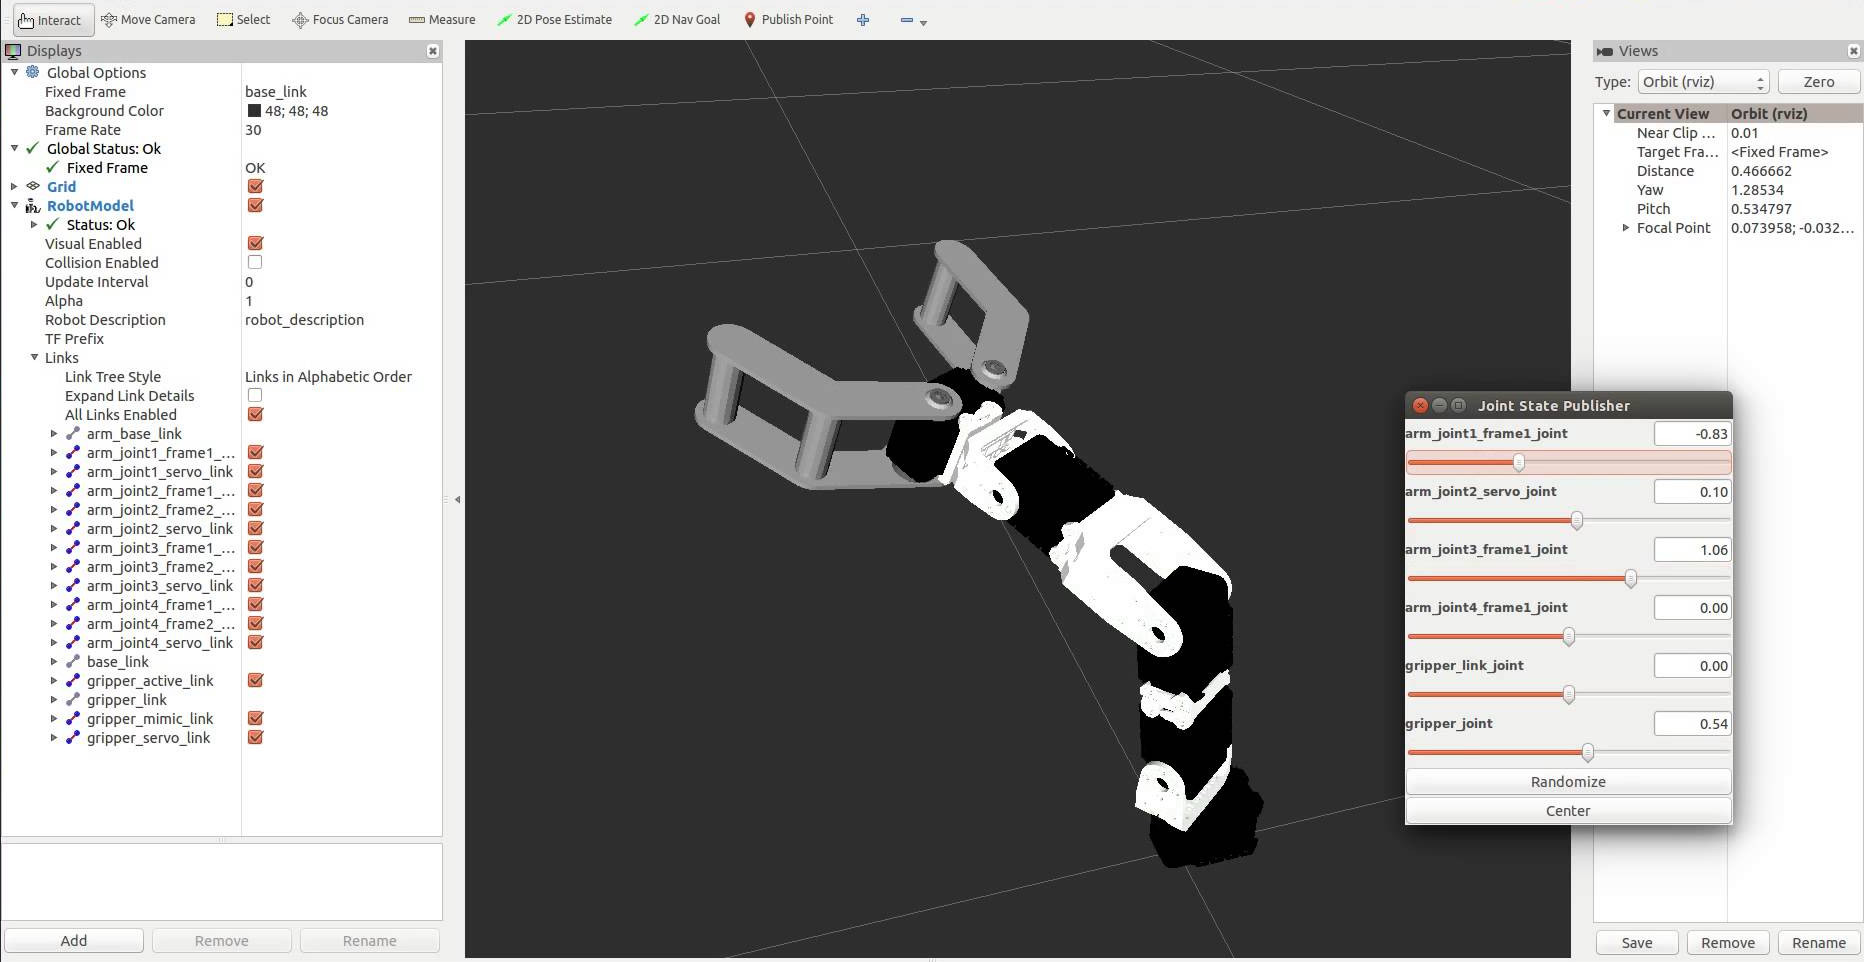
\includegraphics[width=0.8\linewidth]{arm-rviz}
    \end{center}

    3 weeks to:

    \begin{itemize}
        \item Design and build a 3DoF (one stepper, 2 servos) robot arm
        \item Create a 3D model and visualise it
        \item Control it with ROS
    \end{itemize}

\end{frame}

\section[]{"Homework"}

\miniframesoff

\imageframe[scale=0.95]{survey/linux}
\imageframe[scale=0.95]{survey/code}
\imageframe[scale=0.95]{survey/boards}
\imageframe[scale=0.95]{survey/tools}

\miniframeson

\begin{frame}{"Homework"}
    \begin{itemize}
        \item<+-> Thinker with hardware and software!
        \item<+-> \textbf{Write code}, a lot of code -- preferably Python and C++ \\
                I am happy to answer code-related questions
        \item<+-> Invest \textsterling 30 and get a Arduino/RaspberryPI starter kit (like the \href{https://www.amazon.co.uk/s?merchant=A3DM8VCGJL5PKR&fallThrough=1}{Freenove ones})
        \item<+-> \textbf{Make it fun}: come up with \textbf{small, rewarding projects} -- Tetris anyone?
        \item<+-> \textbf{Install Linux} (and use it!) -- alongside Windows as a dualboot, or inside a VM
        \item<+-> Get involved in an \textbf{open-source project}

    \end{itemize}
\end{frame}


\begin{frame}{Attention: I am away on the 11th of October}
    \begin{itemize}
        \item On 11th October: no lecture
        \item On 12th October: practical with Jake
    \end{itemize}
\end{frame}

%%%%%%%%%%%%%%%%%%%%%%%%%%%%%%%%%%%%%%%%%%%%%%%%%%%%%%%%%%%%%%%%%%%%%%%
\miniframesoff
\begin{frame}[plain]
    \begin{center}
        \Large
        10 min break, and off we start!\\[2em]
    \end{center}
\end{frame}
\miniframeson

%%%%%%%%%%%%%%%%%%%%%%%%%%%%%%%%%%%%%%%%%%%%%%%%%%%%%%%%%%%%%%%%%%%%%%%
%%%%%%%%%%%%%%%%%%%%%%%%%%%%%%%%%%%%%%%%%%%%%%%%%%%%%%%%%%%%%%%%%%%%%%%
%%%%%%%%%%%%%%%%%%%%%%%%%%%%%%%%%%%%%%%%%%%%%%%%%%%%%%%%%%%%%%%%%%%%%%%
%%%%%%%%%%%%%%%%%%%%%%%%%%%%%%%%%%%%%%%%%%%%%%%%%%%%%%%%%%%%%%%%%%%%%%%

\section[Arduino]{Intro to Arduino}


\begin{frame}{The Arduino microcontroller}
    \begin{columns}
        \begin{column}{0.5\linewidth}
            \begin{itemize}
                \item What is an Arduino board?
                \item Developing programs
                \item Inputs and outputs
                \item Running control loops
                \item Using PWM to control motors
            \end{itemize}
        \end{column}
        \begin{column}{0.5\linewidth}
            \begin{center}
                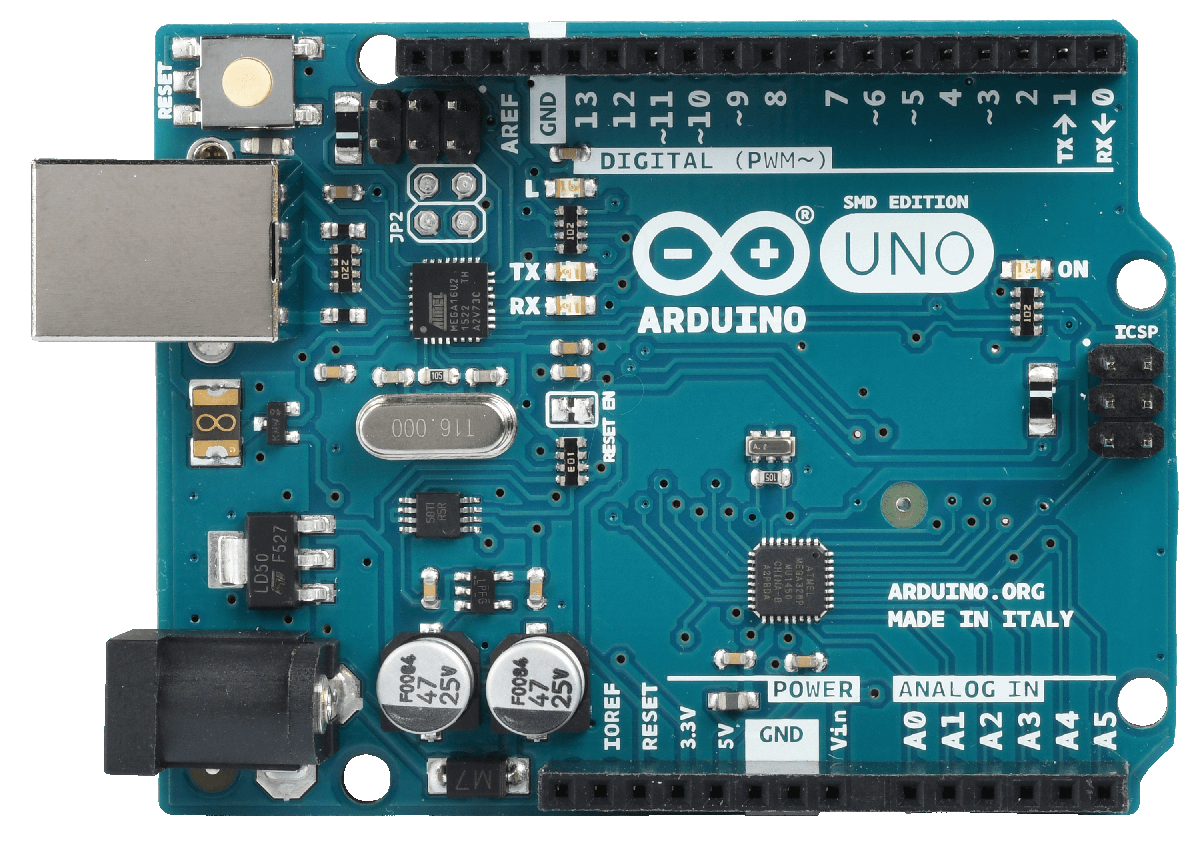
\includegraphics[width=0.8\linewidth]{arduino-uno}
            \end{center}
        \end{column}
    \end{columns}

    \pause

    \begin{itemize}
        \item Arduino is an open-source electronics platform based on easy to
            use hardware and software
        \item it is intended for anyone making interactive projects
        \item very relevant to robotics, including professional-grade projects!
    \end{itemize}
\end{frame}


\begin{frame}{The Arduino microcontroller ecosystem}
    \begin{columns}
        \begin{column}{0.3\linewidth}
            \begin{center}
                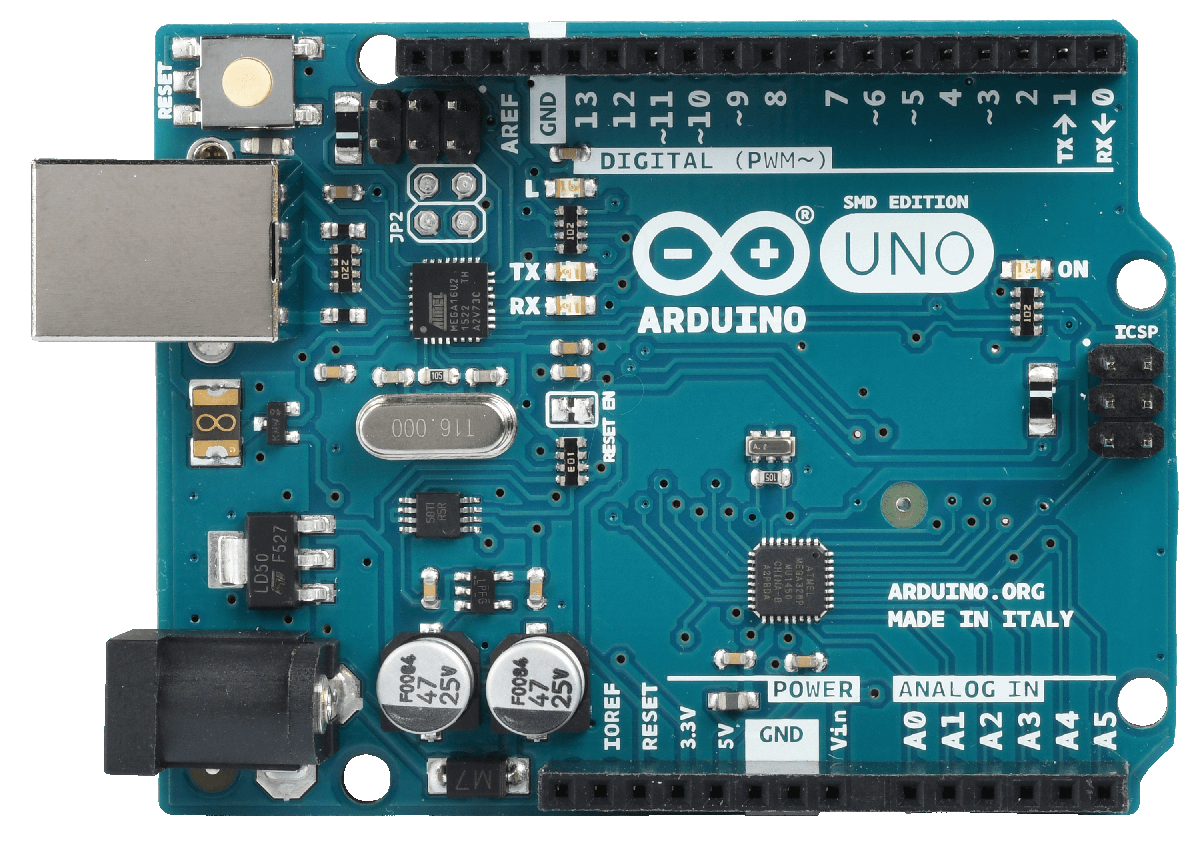
\includegraphics[width=\linewidth]{arduino-uno}\\
                Controller
            \end{center}
        \end{column}
        \begin{column}{0.3\linewidth}
            \begin{center}
                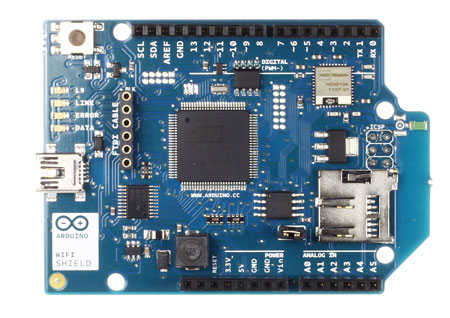
\includegraphics[width=\linewidth]{wifi-shield}\\
                Wifi shield
            \end{center}

        \end{column}
        \begin{column}{0.3\linewidth}
            \begin{center}
            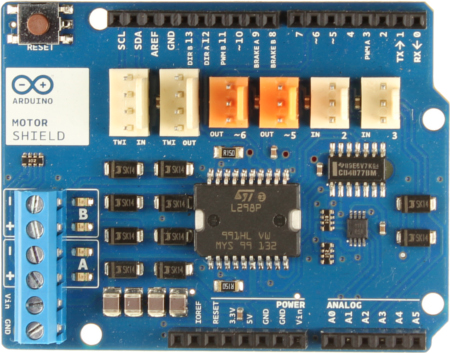
\includegraphics[width=\linewidth]{motor-shield}\\
            Motor shield
            \end{center}

        \end{column}
    \end{columns}

    \vspace{0.5em}

    \begin{columns}
        \begin{column}{0.25\linewidth}
            \begin{center}
                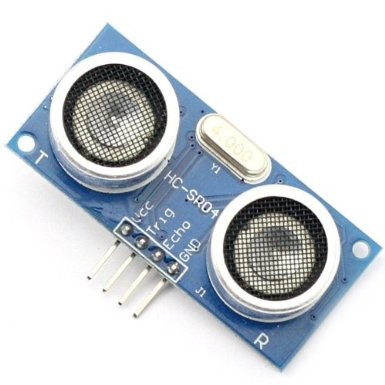
\includegraphics[width=0.9\linewidth]{us-sensor}\\
                Ultrasonic sensor
            \end{center}
        \end{column}
        \begin{column}{0.25\linewidth}
            \begin{center}
                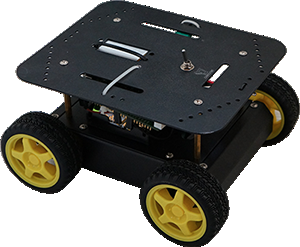
\includegraphics[width=0.9\linewidth]{robot-car}\\
                Robot car
            \end{center}
        \end{column}
         \begin{column}{0.5\linewidth}
             "Arduino is an open-source electronics prototyping
             platform based on flexible,
             easy-to-use hardware and
             software. It's intended for
             artists, designers, hobbyists
             and anyone interested in
             creating interactive objects
             or environments"
        \end{column}
    \end{columns}
\end{frame}

\imageframe[color=white, scale=0.95]{arduino-boards}

\begin{frame}{Arduino Uno}
    \begin{columns}
        \begin{column}{0.5\linewidth}
            \begin{itemize}
                \item Relatively robust board
                \item Microcontroller board based on the ATmega328
                \item 14 digital Input/Output pins
                \item 6 outputs can be used as PWM outputs
                \item 6 analog inputs
                \item 16MHz ceramic resonator
                \item USB connection
                \item power jack
                \item ICSP header
                \item reset button
            \end{itemize}

        \end{column}
        \begin{column}{0.5\linewidth}
            \begin{center}
                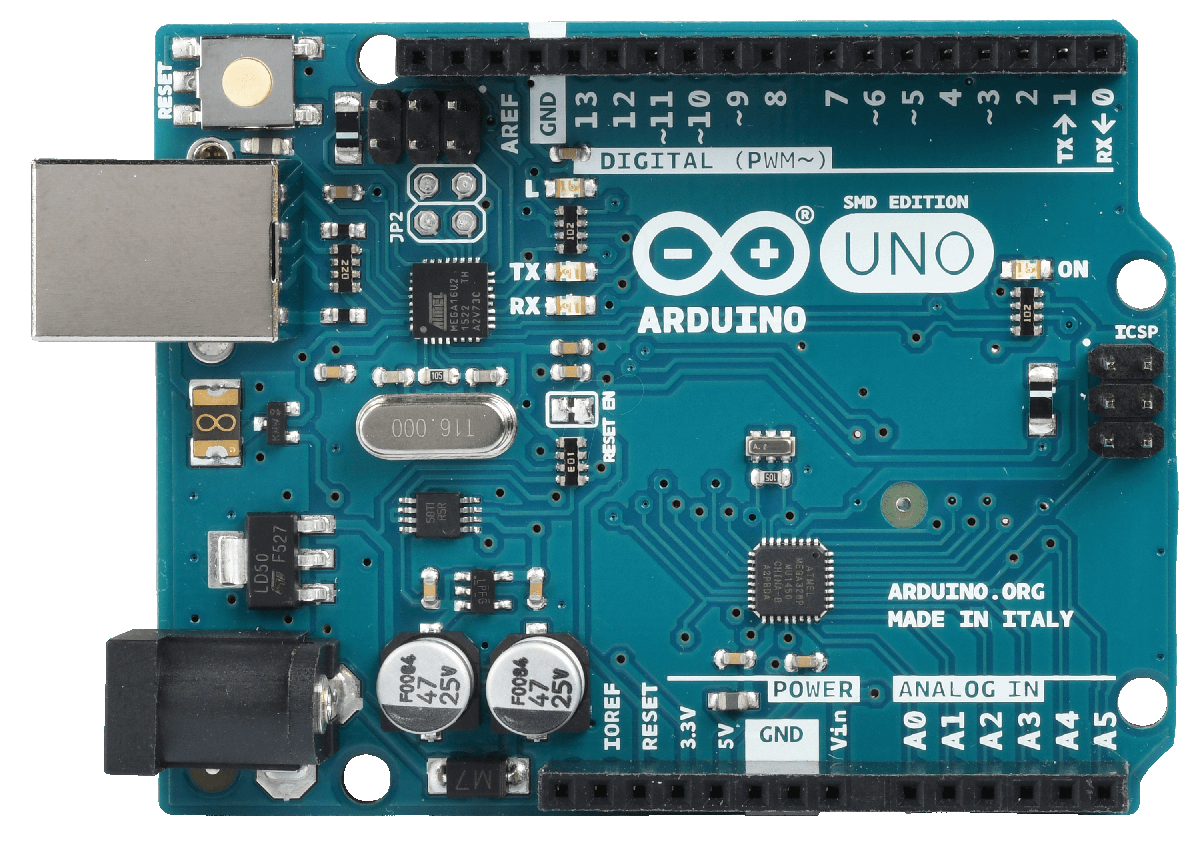
\includegraphics[width=\linewidth]{arduino-uno}
            \end{center}
        \end{column}
    \end{columns}
\end{frame}

\begin{frame}{Arduino Uno}
    \begin{center}
        \includegraphics<1>[width=\linewidth]{arduino-labeled}
        \includegraphics<2>[width=\linewidth]{arduino-labeled-photo}
    \end{center}
\end{frame}

\imageframe{arduino-schematic}

\begin{frame}{Arduino Uno summary}
    \begin{itemize}
        \item Microcontroller: \textbf{ATMega328}
        \item Operating voltage: \textbf{5V}
        \item External input voltage (recommended): 7-12V
        \item External input voltage (limits): \textbf{6-20V}
    \end{itemize}

    \begin{itemize}
        \item Digital I/O pins: 14, of which 6 provide PWM output
        \item Analog input pins: 6
        \item DC current per I/O pin: 40 mA
        \item DC current for 3.3V pin: 50mA
        \item pins have internal pull-up resistors (off by default) of 20-50 k$\Omega$
    \end{itemize}

    \begin{itemize}
        \item RAM: \textbf{2KB}
        \item Flash memory: \textbf{32KB}, of which 0.5KB used by boot loader
        \item EEPROM: 1KB
        \item Clock speed: \textbf{16MHz}
    \end{itemize}
\end{frame}

\begin{frame}[fragile]{What is a pull-up resistor?}

    Prevent \emph{floating} values on the input pins.

    \begin{center}
        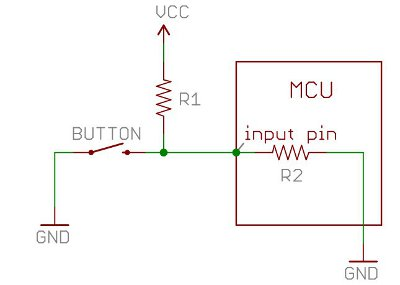
\includegraphics[width=0.5\linewidth]{pullup}
    \end{center}

    The ATmega328 microcontroller has internal pull-ups that can be enabled and disabled:

    \begin{cppcode}
    pinMode(5, INPUT_PULLUP); // Enable internal pull-up resistor on pin 5
    \end{cppcode}

\end{frame}



\begin{frame}{Powering Arduino Uno}
    \begin{itemize}
        \item via the USB connection
        \item external power supply
        \item the power source is selected automatically
        \item external (non-USB) 2.1mm centre-positive plug into the board's
            power jack
        \item leads from a battery can be inserted in the \texttt{Gnd} and
            \texttt{Vin} pin
            headers of the \texttt{POWER} connector
        \item recommended range is 7 to 12 volts
    \end{itemize}
\end{frame}

\begin{frame}{Power comparison}
\begin{tabular}{@{}ll@{}}
\toprule
\textbf{Board}   & \textbf{Power Consumption}           \\ \midrule
RaspberryPI A+   & 80 mA (0.4W)                         \\
RaspberryPI A+   & 160 mA (0.8W) with Wifi dongle       \\
RaspberryPI B+   & 180 mA (0.9W)                        \\
RaspberryPI2 B   & 200 mA (1.0W)                        \\
RaspberryPI Zero & 80 mA (0.4W)                         \\
RaspberryPI Zero & 120 mA (0.7W)                        \\
Arduino Uno      & 30-50mA, can go down to \textless1mA \\ \bottomrule
\end{tabular}

\vspace{1em}
$\rightarrow$ \href{http://www.home-automation-community.com/arduino-low-power-how-to-run-atmega328p-for-a-year-on-coin-cell-battery/}{Arduino for a year on a coin cell}

\end{frame}

\begin{frame}{Some pins have specialized functions}
    \begin{columns}
        \begin{column}{0.5\linewidth}
    \begin{center}
        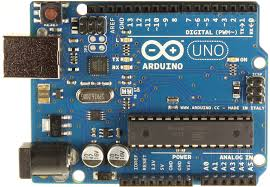
\includegraphics[width=\linewidth]{arduino}
    \end{center}


        \end{column}
        \begin{column}{0.5\linewidth}
    \only<1> {
    \begin{itemize}
        \item Serial: 0 (\texttt{RX}) and 1 (\texttt{TX}) \\
                Used to receive (\texttt{RX}) and transmit (\texttt{TX}) TTL
                serial data
        \item external interrupts: 2 and 3 \\
                Can be configured to trigger an interrupt on a low value, a
                rising or falling edge, or a change in value
        \item PWM: 3, 5, 6, 9, 10 and 11 \\
                Provide 8-bit PWM output with the \cpp{analogWrite()} function
    \end{itemize}
}
    \only<2> {
        \begin{itemize}
            \item SPI: 10 (\texttt{SS}), 11 (\texttt{MOSI}), 12 (\texttt{MISO}),
                13 (\texttt{SCK}) \\
                 Support SPI communication using the SPI library
            \item LED: 13. Built-in LED connected to digital pin 13
            \item The Uno has 6 analog inputs, labeled \texttt{A0} through
                \texttt{A5}
            \item I$^2$C: \texttt{A4} or \texttt{SDA} pin and \texttt{A5} or
                \texttt{SCL} pin \\
                  Support I$^2$C communication using the \texttt{Wire} library
        \end{itemize}
    }
        \end{column}
    \end{columns}
\end{frame}

\begin{frame}{How to start coding: software setup}
    \begin{columns}
        \begin{column}{0.5\linewidth}
            \begin{center}
                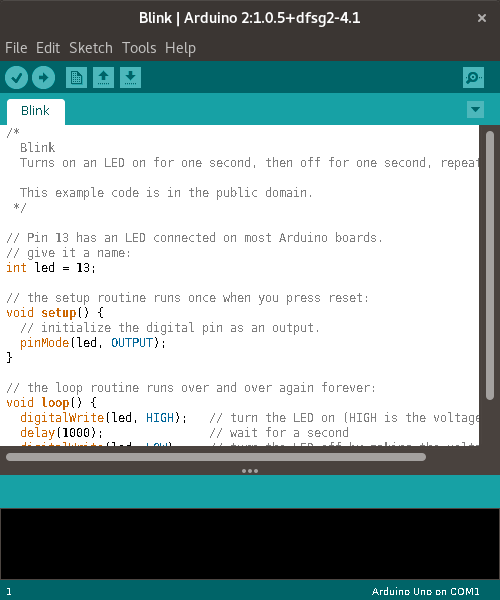
\includegraphics[width=0.9\linewidth]{arduino-ide}
            \end{center}
        \end{column}
        \begin{column}{0.5\linewidth}
            \begin{itemize}
                \item install the IDE (download from \url{www.arduino.cc} or
                    \sh{apt install arduino})
                \item open the Arduino IDE
                \item use a USB A to B cable to plug the board into your
                    computer
                \item setup the board type and serial port from the
                    \emph{Tools} menu
            \end{itemize}
        \end{column}
    \end{columns}
\end{frame}

\begin{frame}{Programming the Arduino}
    \begin{itemize}
        \item Arduino's programming language is a version of C++ with a bit
            of magic (pre-processing) to make it look simpler

        \item Arduino calls a program a \textbf{sketch}. Sketches are saved
            by default in your \textbf{sketchbook} (cf \emph{File >
            Preferences})
        \item Most C/C++ commands work in the sketch editor
        \item 4 basic components of an Arduino program:
            \begin{itemize}
                \item initialization
                \item setup
                \item loop
                \item user defined functions
            \end{itemize}
        \item Arduino Uno is designed to allow it to be remotely reset by
            software

    \end{itemize}
\end{frame}

\begin{frame}{Programming the Arduino: initialization}
    \begin{itemize}
        \item Include any extra libraries you are using
        \item All variables need to be initialized
        \item \cpp{a=4;} will not work, \cpp{int a=4;} will
        \item Declare variables you will assign later: \cpp{int a, b, c;}
        \item Remember datatypes: \cpp{bool}, \cpp{int}, \cpp{double}, \cpp{float}, \cpp{char}, \cpp{String}...
        \item Full reference: \url{https://www.arduino.cc/en/Reference}
    \end{itemize}
\end{frame}

\begin{frame}[fragile]{Programming the Arduino: setup}
    \begin{itemize}
        \item Initialization for the Arduino board
        \item Usually initiate Serial communication
        \item Usually assign digital pins to input or output
        \item For example:
    \end{itemize}

            \begin{cppcode}
void setup() // 'void' means setup() does not return anything
{
    pinMode(13, OUPUT); // pinMode sets the state of a digital pin,
    pinMode(12, INPUT); // either to OUPUT or to INPUT

    Serial.begin(9600); // initialises a serial console at 9600 bauds
}

            \end{cppcode}
\end{frame}


\begin{frame}[fragile]{Programming the Arduino: main loop}
    \begin{itemize}
        \item The loop is the main portion of your program
        \item The microcontroller runs it forever
        \item For instance:
    \end{itemize}

            \begin{cppcode}
void loop()
{
    digitalWrite(13, HIGH); // set the LED on
    delay(1000);            // wait for one second
    digitalWrite(13, LOW);  // set the LED off
    delay(1000);            // wait for one second
}

            \end{cppcode}
\end{frame}


\begin{frame}[fragile]{Programming the Arduino: user defined functions}

    \only<1>{
    \begin{itemize}
        \item These functions can be called in the loop and are usually
            responses to conditions that are met in the loop
        \item These functions must be declared with a \emph{name}, a
            \emph{return type} and optional \emph{input parameters} with their
            types
    \end{itemize}


    The following function maps a user input \cpp{x} from one range to a new
    range:

}
    \begin{cppcode}
float map(float x,
          float in_min, float in_max, 
          float out_min, float out_max)
{
    return (x - in_min) * (out_max - out_min) / (in_max - in_min) + out_min;
}
    \end{cppcode}

    \only<2> {
    The function is defined over \emph{single precision floating numbers},
    represented by the \cpp{float} C type.

    The \cpp{return} statement defines what the function outputs (here, a
    floating number)

    The curly brackets \cpp{{}} define what is inside the function (the
    function \emph{body}). Curly brackets are generally required to separate
    blocks of code.

    The indentation of the code is up to you and does not matter (contrary to
    other languages like Python!)

    }
\end{frame}

\begin{frame}{Programming the Arduino: digital I/O}

    Each of the 14 digital pins on the Uno can be used as an input or output.

    \begin{itemize}
        \item \cpp{pinMode(<pin>, <mode>)}: set a digital pin as \texttt{INPUT}
            or \texttt{OUTPUT}
        \item \cpp{digitalWrite(<pin>, <state>)}: writes to a digital pin
            \texttt{HIGH} (5V) or \texttt{LOW} (\texttt{GND})
        \item \cpp{digitalRead(<pin>)}: reads digital pin and returns
            \texttt{HIGH} or \texttt{LOW}
    \end{itemize}

\end{frame}


\begin{frame}{Programming the Arduino: analog I/O}
    \begin{itemize}
        \item \cpp{analogReference(<type>)}
            \begin{itemize}
                \item \texttt{DEFAULT}: 5V
                \item \texttt{EXTERNAL}: voltage applied to \texttt{Vref}
                \item \url{http://arduino.cc/en/Reference/AnalogReference}
            \end{itemize}
        \item \cpp{analogRead(<pin>)}: reads voltage on given pin, 10 bits
            resolution (1024 values)
    \end{itemize}

\end{frame}

\begin{frame}{Programming the Arduino: serial communications}
    \begin{itemize}
        \item The ATMega328 provides UART TTL serial communication
        \item Available on the digital pins 0 (\texttt{RX}) and 1 (\texttt{TX})
        \item \texttt{RX} and \texttt{TX} LEDs on the board will flash when data
            is being transmitted via the USB-to-serial chip and the the USB
            connection to the computer
    \end{itemize}

    \begin{itemize}
        \item The Arduino IDE includes a serial monitor
        \item It prints out whatever data is received on the serial port
        \item You can also use it to send data using the keyboard
    \end{itemize}
\end{frame}

\begin{frame}{Programming the Arduino: serial library}
    \begin{itemize}
        \item \cpp{Serial.begin(<baudrate>)}: opens serial port at
            \texttt{baudrate}
        \item \cpp{Serial.available()}: returns the nb of bytes available to
            read
        \item \cpp{Serial.read()}: returns the first byte of incoming serial
            data available (or \texttt{-1} if no data is available)
        \item \cpp{Serial.print(<data>, <format>)}: prints data to the serial
            port as readable ASCII text
         \item \cpp{Serial.println(<data>, <format>)}: prints data to the serial
            port as readable ASCII text and adds a line ending
            
    \end{itemize}

    \url{http://arduino.cc/en/Reference/Serial}
\end{frame}

\begin{frame}[fragile]{Programming the Arduino: control flow}

\begin{columns}
    \begin{column}{0.5\linewidth}
        \begin{cppcode}
if(<variable> <comparison operator> <condition>)
{
    // do something
}
else
{
    // do something else
}
        \end{cppcode}
    \end{column}
    \begin{column}{0.5\linewidth}
        \vspace{1em}

        $\rightarrow$ the MCU checks the condition and responds accordingly.

    \end{column}
\end{columns}

\begin{columns}
    \begin{column}{0.5\linewidth}
         \begin{cppcode}
for(<initialization>; <condition>; <increment>)
{
    // do something
}
        \end{cppcode}
    \end{column}
    \begin{column}{0.5\linewidth}
        \vspace{4em}

        $\rightarrow$ the MCU repeats something for a certain number of time.
        For example, read 500 chars on the serial port.

    \end{column}
\end{columns}
\end{frame}

\begin{frame}{Compiling and uploading code}

    \begin{center}
        \begin{tikzpicture}[>=latex]

            \coordinate (compile) at (-4.5,-0.2);
            \coordinate (upload) at (-4,-0.2);
            \coordinate (serial) at (4.4,-0.2);
            \node at (0,0) {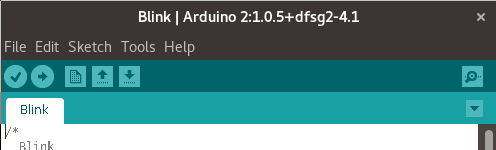
\includegraphics[width=0.9\linewidth]{arduino-ide-detail}};
            \node at (-5,-2) {compile} edge[bend left,ultra thick,double arrow=4pt colored by white and black] (compile);
            \node at (-2.5,-2) {compile + upload} edge[bend right,double arrow=4pt colored by white and black] (upload);
            \node at (3,-2) {serial monitor} edge[bend right,double arrow=4pt colored by white and black] (serial);
        \end{tikzpicture}
    \end{center}



    Under tools, make sure \texttt{Board} matches the actual board you are using and \texttt{Serial port} is the correct one.
\end{frame}

\section[]{Program Examples}

\begin{frame}[fragile]{LED blinking}
    \begin{columns}
        \begin{column}{0.7\linewidth}
\begin{cppcode}
// Pin 13 has an LED connected on most Arduino boards.
// give it a name:
int led = 13;

// the setup routine runs once when you press reset:
void setup() {                
  // initialize the digital pin as an output.
  pinMode(led, OUTPUT);     
}

// the loop routine runs over and over again forever:
void loop() {
  digitalWrite(led, HIGH);   // turn the LED on
  delay(1000);               // wait for a second
  digitalWrite(led, LOW);    // turn the LED off
  delay(1000);               // wait for a second
}
\end{cppcode}

        \end{column}
        \begin{column}{0.3\linewidth}
            \begin{center}
                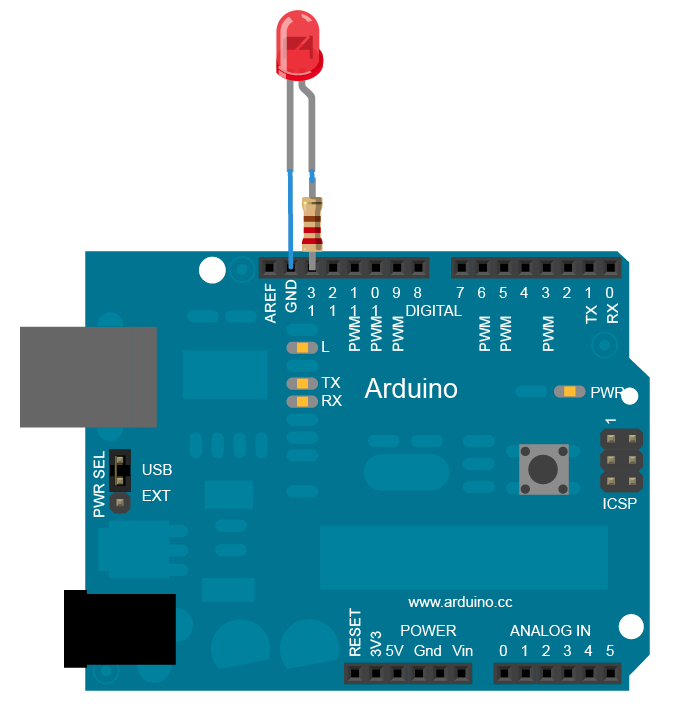
\includegraphics[width=0.35\paperheight]{arduino-led}\\
                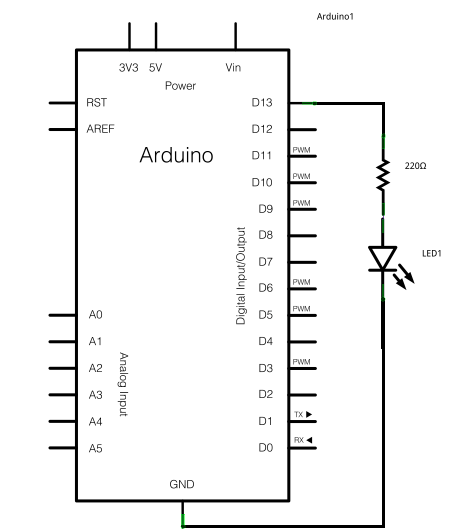
\includegraphics[width=0.3\paperheight]{arduino-led-schematic}
            \end{center}
        \end{column}
    \end{columns}
\end{frame}


\begin{frame}[fragile]{Encoder}
    \begin{columns}
        \begin{column}{0.7\linewidth}
\begin{cppcode}
#include <Encoder.h>

// Change these two numbers to the pins connected to your encoder.
Encoder myEnc(5, 6);
//   avoid using pins with LEDs attached

void setup() {
  Serial.begin(9600);
  Serial.println("Basic Encoder Test:");
}

long oldPosition  = -999;

void loop() {
  long newPosition = myEnc.read();
  if (newPosition != oldPosition) {
    oldPosition = newPosition;
    Serial.println(newPosition);
  }
}
\end{cppcode}

        \end{column}
        \begin{column}{0.3\linewidth}
            \begin{center}
                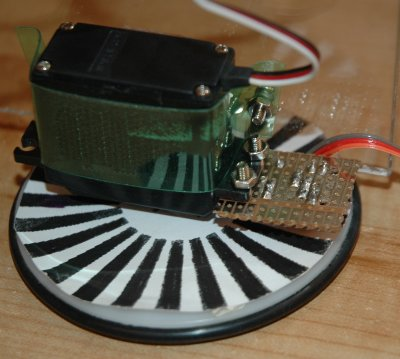
\includegraphics[width=\columnwidth]{encoders3}
            \end{center}
        \end{column}
    \end{columns}
\end{frame}






%%%%%%%%%%%%%%%%%%%%%%%%%%%%%%%%%%%%%%%%%%%%%%%%%%%%%%%%%%%%%%%%%%%%%%%
%%%%%%%%%%%%%%%%%%%%%%%%%%%%%%%%%%%%%%%%%%%%%%%%%%%%%%%%%%%%%%%%%%%%%%%
%%%%%%%%%%%%%%%%%%%%%%%%%%%%%%%%%%%%%%%%%%%%%%%%%%%%%%%%%%%%%%%%%%%%%%%
%%%%%%%%%%%%%%%%%%%%%%%%%%%%%%%%%%%%%%%%%%%%%%%%%%%%%%%%%%%%%%%%%%%%%%%

\section[Encoders]{Measuring position: encoders}

{\fullbackground[scale=0.9,page=2]{ian-sensors.pdf}
    \begin{frame}{Digital incremental encoder}
    \end{frame}
}
{\fullbackground[scale=0.9,page=3]{ian-sensors.pdf}
    \begin{frame}{Optical incremental encoder}
    \end{frame}
}

{\fullbackground[scale=0.9,page=4]{ian-sensors.pdf}
    \begin{frame}{Quadrature output signal generation}
    \end{frame}
}

{\fullbackground[scale=0.9,page=5]{ian-sensors.pdf}
    \begin{frame}{Quadrature output signal usage}
    \end{frame}
}

{\fullbackground[scale=0.9,page=6]{ian-sensors.pdf}
    \begin{frame}{Incremental encoder index signal}
    \end{frame}
}

{\fullbackground[scale=0.9,page=7]{ian-sensors.pdf}
    \begin{frame}{Using all edges increases resolution}
    \end{frame}
}

{\fullbackground[scale=0.9,page=8]{ian-sensors.pdf}
    \begin{frame}{Budget wheel encoders/sensors}
    \end{frame}
}

{\fullbackground[scale=0.9,page=9]{ian-sensors.pdf}
    \begin{frame}{Typical datasheet for encoder}
    \end{frame}
}

{\fullbackground[scale=0.9,page=10]{ian-sensors.pdf}
    \begin{frame}{Absolute optical encoders}
    \end{frame}
}

{\fullbackground[scale=0.9,page=11]{ian-sensors.pdf}
    \begin{frame}{Encoder signal conditioning}
    \end{frame}
}

{\fullbackground[scale=0.9,page=12]{ian-sensors.pdf}
    \begin{frame}{Interface to encoders}
    \end{frame}
}

    \begin{frame}{Interface to Arduino}
        \begin{columns}
            \begin{column}{0.5\linewidth}
                \begin{itemize}
                    \item use interrupt inputs
                    \item count the pulses
                \end{itemize}
            \end{column}
            \begin{column}{0.5\linewidth}
                \begin{center}
                    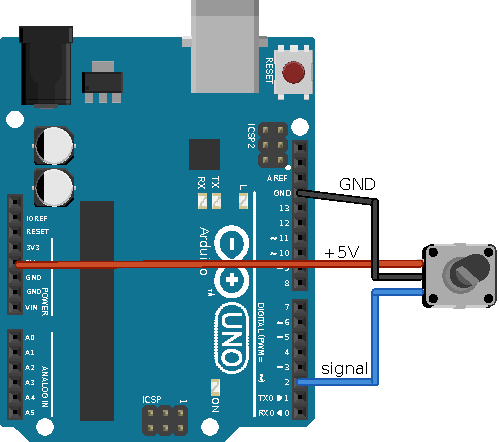
\includegraphics[width=\linewidth]{arduino-encoder}
                \end{center}
            \end{column}
        \end{columns}
    \end{frame}

{\fullbackground[scale=0.9,page=14]{ian-sensors.pdf}
    \begin{frame}{Resolver position measurement}
    \end{frame}
}

{\fullbackground[scale=0.9,page=15]{ian-sensors.pdf}
    \begin{frame}{Resolver position measurement}
    \end{frame}
}

{\fullbackground[scale=0.9,page=16]{ian-sensors.pdf}
    \begin{frame}{Tachometer velocity measurement}
    \end{frame}
}

{\fullbackground[scale=0.9,page=17]{ian-sensors.pdf}
    \begin{frame}{Hall effect magnetic sensor}
    \end{frame}
}

{\fullbackground[scale=0.9,page=18]{ian-sensors.pdf}
    \begin{frame}{Hall effect magnetic sensor circuit}
    \end{frame}
}

{\fullbackground[scale=0.9,page=19]{ian-sensors.pdf}
    \begin{frame}{Hall effect magnetic rotary encoder}
    \end{frame}
}

{\fullbackground[scale=0.9,page=20]{ian-sensors.pdf}
    \begin{frame}{Magnetic rotary encoder}
    \end{frame}
}

{\fullbackground[scale=0.9,page=21]{ian-sensors.pdf}
    \begin{frame}{Electronic commutation systems}
    \end{frame}
}

{\fullbackground[scale=0.9,page=22]{ian-sensors.pdf}
    \begin{frame}{Block commutation}
    \end{frame}
}

{\fullbackground[scale=0.9,page=23]{ian-sensors.pdf}
    \begin{frame}{Components of an EC drive system}
    \end{frame}
}

\miniframesoff
\begin{frame}{}
    \begin{center}
        \Large
        That's all, folks!\\[2em]

            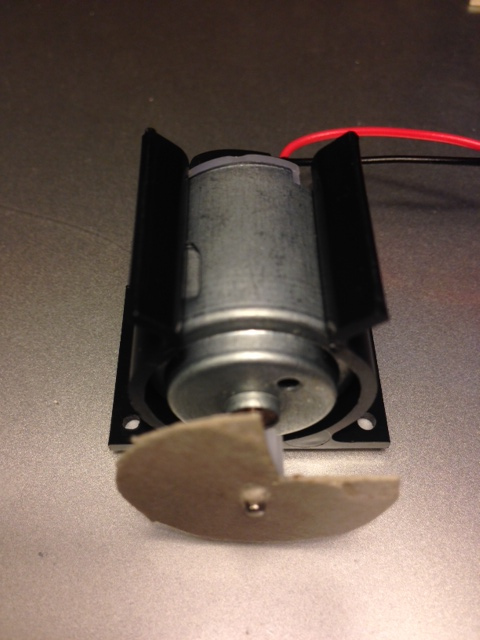
\includegraphics[width=0.25\linewidth]{encoder}

        \normalsize
        \textbf{Questions}:\\
        Portland Square B316 or \url{severin.lemaignan@plymouth.ac.uk} \\[1em]

        \textbf{Slides}:\\
        \href{https://github.com/severin-lemaignan/module-introduction-sensors-actuators}{\small
        github.com/severin-lemaignan/module-introduction-sensors-actuators} \\

        ...or the DLE!


    \end{center}
\end{frame}


\end{document}
